\documentclass[10pt,twocolumn,letterpaper]{article}

\usepackage[margin=0in, paperwidth=1000pt, paperheight=355pt]{geometry}


\usepackage[T1]{fontenc}
\usepackage{times}

\usepackage[font={footnotesize}]{caption}
\usepackage[linesnumbered, ruled]{algorithm2e}
\usepackage[percent]{overpic}
\usepackage{amsmath}
\usepackage{amssymb}
\usepackage{booktabs}
\usepackage{color}
\usepackage{comment}
\usepackage{contour}
\usepackage{dsfont}
\usepackage{floatrow}
\usepackage{graphicx}
\usepackage{layouts}
\usepackage{listings}
\usepackage{multirow}
\usepackage{subcaption}
\usepackage{tabularx}
\usepackage{tcolorbox}
\usepackage{transparent}
\usepackage{url}
\usepackage{verbatim}
\usepackage{xspace}

\usepackage[pagebackref=true,breaklinks=true,letterpaper=true,colorlinks,bookmarks=false]{hyperref}
%\usepackage[capitalise]{cleveref}
\usepackage{cleveref}

\newfloatcommand{capbtabbox}{table}[][\FBwidth]

\newcommand{\mytodo}[1]{{\noindent\textcolor{red}{TODO: #1}}}
\newcommand{\todo}[1]{\mytodo{#1}}
\newcommand{\bbf}{\mathbf{f}}
\newcommand{\bx}{\mathbf{x}}
\newcommand{\by}{\mathbf{y}}
\newcommand{\bz}{\mathbf{z}}
\newcommand{\bw}{\mathbf{w}}
\newcommand{\be}{\mathbf{e}}
\newcommand{\bv}{\mathbf{v}}
\newcommand{\methodname}{Invariant Information Clustering\xspace}
\newcommand{\methodnameshort}{IIC\xspace}
\newcommand{\bdash}{\mathbf{'}}
\newcommand{\bc}{\mathbf{c}}
\newcommand{\defeq}{\overset{\Delta}{=}}
\newcommand{\cmt}[1]{\ignorespaces}

\newcommand{\matP}{\mathbf{P}}  %\boldsymbol{P}

% Default fixed font does not support bold face
\DeclareFixedFont{\ttb}{T1}{txtt}{bx}{n}{6.5} % for bold
\DeclareFixedFont{\ttm}{T1}{txtt}{m}{n}{6.5}  % for normal

% Suppress annoying badness warnings (disable for final version).
\hfuzz=10000pt
\vfuzz=10000pt
\hbadness=2000
\vbadness=\maxdimen

% No space paragraph.
\makeatletter
\renewcommand{\paragraph}{%
  \@startsection{paragraph}{4}%
  %{\z@}{3.25ex \@plus 1ex \@minus .2ex}{-1em}%
  {\z@}{0.5em}{-1em}%
  {\normalfont\normalsize\bfseries}%
}
\makeatother

\DeclareMathOperator*{\argmax}{argmax}
\DeclareMathOperator*{\argmin}{argmin}

% General parameters, for ALL pages:
\renewcommand{\topfraction}{0.9}    % max fraction of floats at top
\renewcommand{\bottomfraction}{0.8} % max fraction of floats at bottom

% Parameters for TEXT pages (not float pages):
\setcounter{topnumber}{2}
\setcounter{bottomnumber}{2}
\setcounter{totalnumber}{4} % 2 may work better
\setcounter{dbltopnumber}{2} % for 2-column pages
\renewcommand{\dbltopfraction}{0.9} % fit big float above 2-col. text
\renewcommand{\textfraction}{0.07} % allow minimal text w. figs

% Parameters for FLOAT pages (not text pages):
\renewcommand{\floatpagefraction}{0.7} % require fuller float pages

% N.B.: floatpagefraction MUST be less than topfraction !!
\renewcommand{\dblfloatpagefraction}{0.7} % require fuller float pages

% Separation between text and figure etc
\setlength{\textfloatsep}{5.0pt plus 2.0pt minus 4.0pt}
\setlength{\floatsep}{5.0pt plus 2.0pt minus 2.0pt}
\setlength{\intextsep}{5.0pt plus 2.0pt minus 2.0pt}
\setlength{\dbltextfloatsep}{5.0pt plus 2.0pt minus 2.0pt}
\setlength{\dblfloatsep}{5.0pt plus 2.0pt minus 2.0pt}

\floatsetup[table]{capposition=bottom,captionskip=0.2em}
\floatsetup[figure]{capposition=bottom,captionskip=0.2em}

\usepackage{rotating}


\begin{document}


%\begin{sideways}
\begin{minipage}{35cm}

\contourlength{1pt} %how thick each copy is
\contournumber{40}  %number of copies
\newcommand{\xput}[3]{%
% \begin{overpic}[#1]{#2}%
% \put (80,5) {\transparent{0.8}{\scriptsize{\colorbox{white}{#3}}}}%
% %\put (5,5) {\scriptsize\makebox(0,0){\contour{white}{#3}}}%
% %\put (5,5) {\scriptsize{\contour{white}{#3}}}%
% \end{overpic}
\includegraphics[#1]{#2}%
\raisebox{12pt}{\makebox[0pt][r]{%
%\transparent{0.8}{\contour{white}{\scriptsize #3\ }}}}}
%\transparent{0.8}{\colorbox{white}{\scriptsize #3}}}}}
\transparent{0.8}{\Large\tcbox[colback=white,size=fbox,on line]{#3}}}}}



\begin{minipage}{0.27\textwidth}
\raggedright
\setlength\tabcolsep{1pt}
\renewcommand{\arraystretch}{0.8}
\begin{tabular}{ccc}
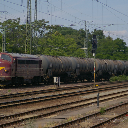
\includegraphics[height=0.32\textwidth]{experiments2_files/509_img_77.png} &
\xput{height=0.32\textwidth}{experiments2_files/509_reordered_preds_77.png}{IIC} &
\xput{height=0.32\textwidth}{experiments2_files/509_targets_77.png}{GT} \\
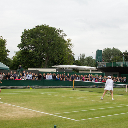
\includegraphics[height=0.32\textwidth]{experiments2_files/509_img_441.png}&
\xput{height=0.32\textwidth}{experiments2_files/509_reordered_preds_441.png}{IIC} &
\xput{height=0.32\textwidth}{experiments2_files/509_targets_441.png}{GT} \\
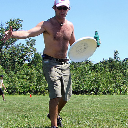
\includegraphics[height=0.32\textwidth]{experiments2_files/496_img_64.png} &
\xput{height=0.32\textwidth}{experiments2_files/496_reordered_preds_64.png}{IIC*} &
\xput{height=0.32\textwidth}{experiments2_files/496_targets_64.png}{GT}  \\
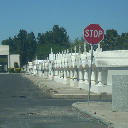
\includegraphics[height=0.32\textwidth]{experiments2_files/496_img_489.png} &
\xput{height=0.32\textwidth}{experiments2_files/496_reordered_preds_489.png}{IIC*} &
\xput{height=0.32\textwidth}{experiments2_files/496_targets_489.png}{GT} \\
\end{tabular}
\end{minipage}~%
\begin{minipage}{0.72\textwidth}
\raggedright
\setlength\tabcolsep{1.2pt}
\begin{tabular}{cccc}
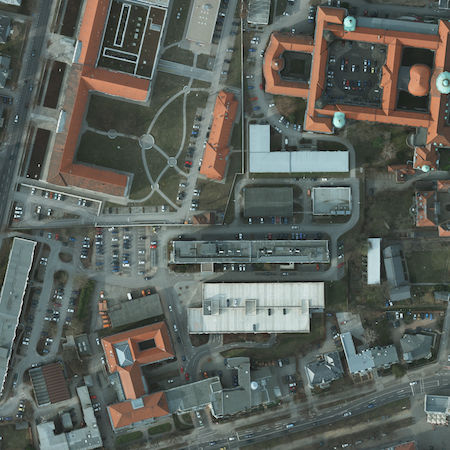
\includegraphics[height=0.243\textwidth]{experiments2_files/545_12_img.png} &
\xput{height=0.243\textwidth}{experiments2_files/545_12_preds.png}{IIC} &
\xput{height=0.243\textwidth}{experiments2_files/482_12_preds.png}{IIC*} &
\xput{height=0.243\textwidth}{experiments2_files/545_12_gt.png}{GT} \\
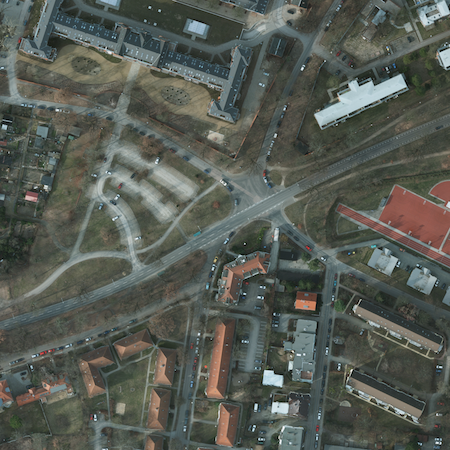
\includegraphics[height=0.243\textwidth]{experiments2_files/545_5_img.png} &
\xput{height=0.243\textwidth}{experiments2_files/545_5_preds.png}{IIC} &
\xput{height=0.243\textwidth}{experiments2_files/482_5_preds.png}{IIC*} &
\xput{height=0.243\textwidth}{experiments2_files/545_5_gt.png}{GT} \\
\end{tabular}
\end{minipage}

\end{minipage}
%\end{sideways}

\end{document}
